% answers.tex —— 1977 年·新疆卷（理科） · 参考答案与详细解析片段
% 由 tools/generate_projects.py 依来源总账自 1977/1977_数学真题_新疆理_试题.md + 1977/1977_数学真题_新疆理_解析正文.md + 1977/1977_数学真题_新疆理_答案要点.md 生成，勿手改（改源 MD 后重跑）


\begin{gktip}
固定源是题面与解答连续出现的扫描材料《新疆 1977 年高考数学试题解（理工科）》（书籍页码 125—127，第 4 页未见页码）。下文逐题独立推导，并对照源解答复核关键结论；源解答两处排印问题在第 1、4 题下加源注。原卷大题「一」至「六」已重排为第 1—6 题，参考题「一」至「四」转录为参考题 1—4；「一」「三」之下的小题已重排为连续小问（1）（2）……。
\end{gktip}

\begin{answer}
\gksolhead{1}{}

\textbf{题目}（每小题 6 分）：

（1） $\operatorname{Log}_3\dfrac{1}{27}=$\mbox{（　　）}；$\operatorname{Log}_{10}(\operatorname{Log}_{10}10)=$\mbox{（　　）}

（2） 当 $a$ 取什么值时，方程 $x^2-2x+\operatorname{Lg}a=0$ 有实数根。

\Needspace{5\baselineskip}
（3） 解方程：

\nopagebreak[4]
\[
7^{2x^2+x-6}=1.
\]

（4） 求等比数列 $\sqrt[6]{3}$，$\sqrt[3]{3}$，$\sqrt{3}$，…… 的公比 $q$，并写出它的第六项 $a_6$。

\Needspace{4\baselineskip}
\textbf{解析}

\gksubpart{（1）}

$\log_3\dfrac{1}{27}=\log_3 3^{-3}=-3$，故第一空为 $-3$；又 $\log_{10}(\log_{10}10)=\log_{10}1=0$，故第二空为 $0$。

\begin{gktip}
\textbf{源注}：源解答此空印作「$\operatorname{Log}_3\frac{1}{27}=\frac{1}{27}$」，与 $\log_3\frac{1}{27}=-3$ 不符，系排印错误；同句第二空 $\operatorname{Log}_{10}(\operatorname{Log}_{10}10)=0$ 印刷正确。
\end{gktip}

\gksubpart{（2）}

\Needspace{5\baselineskip}
方程 $x^2-2x+\lg a=0$ 有实数根，须判别式非负：

\nopagebreak[4]
\[
\Delta=(-2)^2-4\lg a\ge0
\quad\Longrightarrow\quad
\lg a\le1
\quad\Longleftrightarrow\quad
a\le10.
\]

又对数的真数须为正，即 $a>0$，故当 $0<a\le10$ 时方程有实数根。

\gksubpart{（3）}

\Needspace{5\baselineskip}
由 $7^{2x^2+x-6}=1=7^0$ 得

\nopagebreak[4]
\[
2x^2+x-6=0,
\qquad
(2x-3)(x+2)=0,
\]

\Needspace{5\baselineskip}
所以

\nopagebreak[4]
\[
x_1=\frac32\ \text{（\text{即}}\ 1\tfrac12\text{）},
\qquad
x_2=-2.
\]

\gksubpart{（4）}

\Needspace{5\baselineskip}
$a_1=\sqrt[6]{3}=3^{1/6}$，$a_2=\sqrt[3]{3}=3^{2/6}$，$a_3=\sqrt{3}=3^{3/6}$，确实构成公比 $q=3^{1/6}$ 的等比数列。于是

\nopagebreak[4]
\[
q=\frac{\sqrt[3]{3}}{\sqrt[6]{3}}
=\frac{\sqrt[6]{3^2}}{\sqrt[6]{3}}
=\sqrt[6]{3}.
\]

\Needspace{5\baselineskip}
第六项

\nopagebreak[4]
\[
a_6=a_1q^5
=\sqrt[6]{3}\cdot\bigl(\sqrt[6]{3}\bigr)^5
=3^{1/6+5/6}=3.
\]

\gkanswer{答案（1）：$-3$；$0$。}

\gkanswer{答案（2）：$0<a\le10$。}

\gkanswer{答案（3）：$x_1=\dfrac32$，$x_2=-2$。}

\gkanswer{答案（4）：$q=\sqrt[6]{3}$，$a_6=3$。}

\end{answer}
\begin{answer}
\gksolhead{2}{}

\textbf{题目}（16 分）：

在底边为 2 尺，高为 1.6 尺的三角形内截一个最大面积的矩形，并使其一边在三角形的底边上，求矩形的长和宽各是多少？
\nopagebreak[4]
\begin{center}% 1977 年新疆卷（理科）第二题：三角形 ABC 内截矩形 EFGH，一边 FG 在 BC 上，
% AD 为 BC 边上的高，K 为 AD 与 EH 的交点（按源卷第 2 页布局）
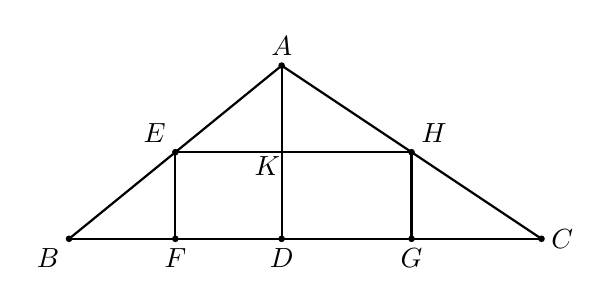
\begin{tikzpicture}[scale=1]
  \coordinate (B) at (0,0);
  \coordinate (C) at (6,0);
  \coordinate (A) at (2.7,2.2);
  \coordinate (D) at (2.7,0);
  \coordinate (E) at (1.35,1.1);
  \coordinate (H) at (4.35,1.1);
  \coordinate (F) at (1.35,0);
  \coordinate (G) at (4.35,0);
  \coordinate (K) at (2.7,1.1);
  \draw[thick] (B)--(C);
  \draw[thick] (A)--(B);
  \draw[thick] (A)--(C);
  \draw[thick] (A)--(D);
  \draw[thick] (E)--(H);
  \draw[thick] (E)--(F);
  \draw[thick] (H)--(G);
  \fill (A) circle (1.2pt) node[above] {$A$};
  \fill (B) circle (1.2pt) node[below left] {$B$};
  \fill (C) circle (1.2pt) node[right] {$C$};
  \fill (D) circle (1.2pt) node[below] {$D$};
  \fill (E) circle (1.2pt) node[above left] {$E$};
  \fill (F) circle (1.2pt) node[below] {$F$};
  \fill (G) circle (1.2pt) node[below] {$G$};
  \fill (H) circle (1.2pt) node[above right] {$H$};
  \node at (2.52,0.92) {$K$};
\end{tikzpicture}
\end{center}
\nopagebreak[4]
\Needspace{4\baselineskip}
\textbf{解析}
\nopagebreak[4]
\begin{center}% 1977 年新疆卷（理科）第二题：三角形 ABC 内截矩形 EFGH，一边 FG 在 BC 上，
% AD 为 BC 边上的高，K 为 AD 与 EH 的交点（按源卷第 2 页布局）
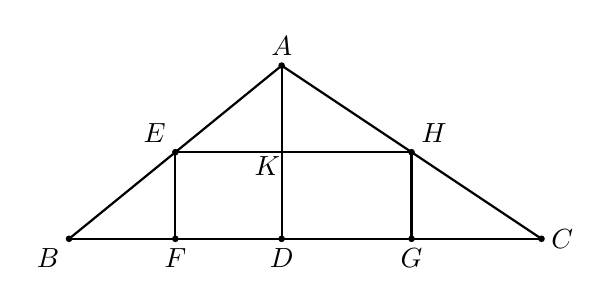
\begin{tikzpicture}[scale=1]
  \coordinate (B) at (0,0);
  \coordinate (C) at (6,0);
  \coordinate (A) at (2.7,2.2);
  \coordinate (D) at (2.7,0);
  \coordinate (E) at (1.35,1.1);
  \coordinate (H) at (4.35,1.1);
  \coordinate (F) at (1.35,0);
  \coordinate (G) at (4.35,0);
  \coordinate (K) at (2.7,1.1);
  \draw[thick] (B)--(C);
  \draw[thick] (A)--(B);
  \draw[thick] (A)--(C);
  \draw[thick] (A)--(D);
  \draw[thick] (E)--(H);
  \draw[thick] (E)--(F);
  \draw[thick] (H)--(G);
  \fill (A) circle (1.2pt) node[above] {$A$};
  \fill (B) circle (1.2pt) node[below left] {$B$};
  \fill (C) circle (1.2pt) node[right] {$C$};
  \fill (D) circle (1.2pt) node[below] {$D$};
  \fill (E) circle (1.2pt) node[above left] {$E$};
  \fill (F) circle (1.2pt) node[below] {$F$};
  \fill (G) circle (1.2pt) node[below] {$G$};
  \fill (H) circle (1.2pt) node[above right] {$H$};
  \node at (2.52,0.92) {$K$};
\end{tikzpicture}
\end{center}
\nopagebreak[4]
\Needspace{5\baselineskip}
设矩形下边 $FG$ 在 $BC$ 上，上边 $EH\parallel BC$，$\triangle ABC$ 的高 $AD$ 与 $EH$ 交于 $K$。由 $EH\parallel BC$ 得 $\triangle AEH\sim\triangle ABC$，从而

\nopagebreak[4]
\[
\frac{EH}{BC}=\frac{AK}{AD}.
\]

\Needspace{5\baselineskip}
设矩形的长 $EH=x$ 尺，则 $\dfrac{x}{2}=\dfrac{AK}{1.6}$，得 $AK=0.8x$。矩形的宽

\nopagebreak[4]
\[
HG=KD=AD-AK=1.6-0.8x.
\]

\Needspace{5\baselineskip}
面积

\nopagebreak[4]
\[
S=x(1.6-0.8x)
=-0.8x^2+1.6x
=-0.8(x-1)^2+0.8.
\]

所以当 $x=1$ 时 $S$ 最大，此时 $HG=KD=1.6-0.8\times1=0.8$ 尺。即矩形长 $1$ 尺、宽 $0.8$ 尺。

\gkanswer{答案：长 $1$ 尺，宽 $0.8$ 尺。}

\end{answer}
\begin{answer}
\gksolhead{3}{}

\textbf{题目}：

（1） 求 $\operatorname{ctg}(-1200^\circ)$ 的值。（6 分）

（2） 已知 $\sin\alpha=-\dfrac{12}{13}$，并且 $\pi<\alpha<\dfrac{3\pi}{2}$，求 $\cos\dfrac{\alpha}{2}$。

\Needspace{4\baselineskip}
\textbf{解析}

\gksubpart{（1）}

\nopagebreak[4]
\[
\operatorname{ctg}(-1200^\circ)
=-\operatorname{ctg}1200^\circ
=-\operatorname{ctg}(360^\circ\times3+120^\circ)
=-\operatorname{ctg}120^\circ
\]

\Needspace{5\baselineskip}
再由 $120^\circ=180^\circ-60^\circ$ 与 $\operatorname{ctg}(180^\circ-\theta)=-\operatorname{ctg}\theta$，

\nopagebreak[4]
\[
-\operatorname{ctg}120^\circ
=-\operatorname{ctg}(180^\circ-60^\circ)
=\operatorname{ctg}60^\circ
=\frac{\sqrt3}{3}.
\]

\gksubpart{（2）}

\Needspace{5\baselineskip}
由 $\pi<\alpha<\dfrac{3\pi}{2}$ 得 $\dfrac{\pi}{2}<\dfrac{\alpha}{2}<\dfrac{3\pi}{4}$，故 $\cos\dfrac{\alpha}{2}$ 为负值。先求

\nopagebreak[4]
\[
\cos\alpha
=-\sqrt{1-\sin^2\alpha}
=-\sqrt{1-\Bigl(-\frac{12}{13}\Bigr)^2}
=-\frac{5}{13}.
\]

\Needspace{5\baselineskip}
再用半角公式取负根：

\nopagebreak[4]
\[
\cos\frac{\alpha}{2}
=-\sqrt{\frac{1+\cos\alpha}{2}}
=-\sqrt{\frac{1-\frac{5}{13}}{2}}
=-\sqrt{\frac{4}{13}}
=-\frac{2\sqrt{13}}{13}.
\]

\gkanswer{答案（1）：$\dfrac{\sqrt3}{3}$。}

\gkanswer{答案（2）：$-\dfrac{2\sqrt{13}}{13}$。}

\end{answer}
\begin{answer}
\gksolhead{4}{}

\textbf{题目}（12 分）：

三角形的三边长分别是 4 cm，5 cm，$\sqrt{61}$ cm，求这个三角形内最大角的度数。

\Needspace{4\baselineskip}
\textbf{解析}

\Needspace{5\baselineskip}
最大角对最长边：三边 $4$、$5$、$\sqrt{61}$ 中 $\sqrt{61}\approx7.81$ 最长，其对角 $\alpha$ 即最大角。由余弦定理，

\nopagebreak[4]
\[
\cos\alpha=\frac{4^2+5^2-(\sqrt{61})^2}{2\times4\times5}
=\frac{16+25-61}{40}
=-\frac12,
\]

\Needspace{5\baselineskip}
故

\nopagebreak[4]
\[
\alpha=120^\circ.
\]

\begin{gktip}
\textbf{源注}：源解答此式印作「$\cos\alpha=-\dfrac{-(\sqrt{61})^2+4^2+5^2}{2\times4\times5}$」，分式外多印一个负号，与其后「$=\dfrac{-61+16+25}{40}=-\dfrac12$」自相矛盾；按余弦定理分式前不应有负号，数值结论不变。
\end{gktip}

\gkanswer{答案：$120^\circ$。}

\end{answer}
\begin{answer}
\gksolhead{5}{}

\textbf{题目}（18 分）：

求经过园 $2x^2-20x+2y^2+18=0$ 上一点 $p(3,\ 2\sqrt3)$ 的切线方程。

\begin{gktip}
\textbf{源注}：原卷「圆」印作「园」（第六题「园弧」、参考题四「椭园」同），本文按原卷用字保留。
\end{gktip}

\Needspace{4\baselineskip}
\textbf{解析}

\Needspace{5\baselineskip}
圆 $2x^2-20x+2y^2+18=0$ 两边除以 $2$：

\nopagebreak[4]
\[
x^2+y^2-10x+9=0,
\qquad\text{\text{即}}\qquad
(x-5)^2+y^2=16,
\]

圆心 $(5,0)$，半径 $4$。点 $p(3,\ 2\sqrt3)$ 代入左端得 $9+12-30+9=0$，确在圆上。

\Needspace{5\baselineskip}
半径 $Op$ 的斜率 $k_1=\dfrac{2\sqrt3-0}{3-5}=-\sqrt3$，切线与半径垂直，斜率 $k=\dfrac{1}{\sqrt3}$。切线方程

\nopagebreak[4]
\[
y-2\sqrt3=\frac{1}{\sqrt3}(x-3),
\]

\Needspace{5\baselineskip}
两边乘 $\sqrt3$ 化简得

\nopagebreak[4]
\[
\sqrt3\,y-x-3=0.
\]

\gkanswer{答案：$\sqrt3\,y-x-3=0$。}

\end{answer}
\begin{answer}
\gksolhead{6}{}

\textbf{题目}（14 分）：

园弧拱桥的拱坡跨径 $AB=16$ 米，主拱高为 2.5 米，计算 $\overset{\frown}{AB}$ 的半径是多少米？
\nopagebreak[4]
\begin{center}% 1977 年新疆卷（理科）第六题：圆弧拱桥，弦 AB 为跨径，C 为拱顶，
% CD⊥AB 为主拱高，CD 延长线过圆心 O，OB=R（按源卷第 3 页布局）
\begin{tikzpicture}[scale=0.72]
  \coordinate (A) at (0,0);
  \coordinate (B) at (8,0);
  \coordinate (C) at (4,1.25);
  \coordinate (D) at (4,0);
  \coordinate (O) at (4,-5.775);
  \draw[thick] (A) arc[start angle=124.68, end angle=55.32, radius=7.025];
  \draw[thick] (A)--(B);
  \draw[dashed,->] (C)--(O);
  \draw[dashed,->] (B)--(O);
  \fill (A) circle (1.2pt) node[below left] {$A$};
  \fill (B) circle (1.2pt) node[right] {$B$};
  \fill (C) circle (1.2pt) node[above left] {$C$};
  \fill (D) circle (1.2pt) node[below left] {$D$};
  \fill (O) circle (1.2pt) node[below] {$O$};
  \node[right] at (6,-2.89) {$R$};
\end{tikzpicture}
\end{center}
\nopagebreak[4]
\begin{gktip}
\textbf{参考题}
\end{gktip}

\Needspace{5\baselineskip}
\textbf{参考题 1．} 解方程：

\nopagebreak[4]
\[
\operatorname{Log}_{16-3x}(x-2)=\operatorname{Log}_8 2\sqrt2.
\]

\Needspace{5\baselineskip}
\textbf{参考题 2．} 已知 $0^\circ<x<45^\circ$，且有

\nopagebreak[4]
\[
\operatorname{Lg}\operatorname{tg}x-\operatorname{Lg}\sin x
=\operatorname{Lg}\cos x-\operatorname{Lg}\operatorname{ctg}x
+2\operatorname{Lg}3-\frac{3}{2}\operatorname{Lg}2,
\]

试求 $\sin x-\cos x$ 的值。

\textbf{参考题 3．} 应用导数，求过曲线 $x^2+y^2-8x-2y+12=0$ 上一点 $p(5,\ 3)$ 的切线方程。

\textbf{参考题 4．} 利用定积分，求椭园 $4x^2+25y^2=100$ 的面积。

\Needspace{4\baselineskip}
\textbf{解析}
\nopagebreak[4]
\begin{center}% 1977 年新疆卷（理科）第六题：圆弧拱桥，弦 AB 为跨径，C 为拱顶，
% CD⊥AB 为主拱高，CD 延长线过圆心 O，OB=R（按源卷第 3 页布局）
\begin{tikzpicture}[scale=0.72]
  \coordinate (A) at (0,0);
  \coordinate (B) at (8,0);
  \coordinate (C) at (4,1.25);
  \coordinate (D) at (4,0);
  \coordinate (O) at (4,-5.775);
  \draw[thick] (A) arc[start angle=124.68, end angle=55.32, radius=7.025];
  \draw[thick] (A)--(B);
  \draw[dashed,->] (C)--(O);
  \draw[dashed,->] (B)--(O);
  \fill (A) circle (1.2pt) node[below left] {$A$};
  \fill (B) circle (1.2pt) node[right] {$B$};
  \fill (C) circle (1.2pt) node[above left] {$C$};
  \fill (D) circle (1.2pt) node[below left] {$D$};
  \fill (O) circle (1.2pt) node[below] {$O$};
  \node[right] at (6,-2.89) {$R$};
\end{tikzpicture}
\end{center}
\nopagebreak[4]
\Needspace{5\baselineskip}
跨径 $AB=16$ 米即弦 $\overset{\frown}{AB}$ 之弦长，主拱 $CD=2.5$ 米且 $CD\perp AB$，其延长线过圆心 $O$。由垂径定理，$D$ 平分弦，$AD=DB=\frac12AB=8$ 米，$OD=R-2.5$。在 $\mathrm{Rt}\triangle ODB$ 中，

\nopagebreak[4]
\[
R^2=(R-2.5)^2+8^2,
\]

\Needspace{5\baselineskip}
展开得

\nopagebreak[4]
\[
R^2=R^2-5R+6.25+64,
\qquad
5R=70.25,
\qquad
R=14.05\ \text{\text{米}}.
\]

\textbf{参考题 1}

\Needspace{5\baselineskip}
由对数定义，$\operatorname{Log}_8 2\sqrt2=\operatorname{Log}_8 8^{\frac12}=\dfrac12$，故

\nopagebreak[4]
\[
\operatorname{Log}_{16-3x}(x-2)=\frac12
\quad\Longleftrightarrow\quad
(16-3x)^{\frac12}=x-2.
\]

\Needspace{5\baselineskip}
两边平方：

\nopagebreak[4]
\[
16-3x=x^2-4x+4,
\qquad\text{\text{即}}\qquad
x^2-x-12=0,
\qquad
(x-4)(x+3)=0.
\]

解得 $x_1=4$，$x_2=-3$。检验：$x=-3$ 使真数 $x-2=-5<0$，是增根，舍去；$x=4$ 时底 $16-3\times4=4$、真数 $2$，$\operatorname{Log}_4 2=\frac12$ 。故原方程的解是 $x=4$。

\textbf{参考题 2}

\Needspace{5\baselineskip}
利用对数性质合并：

\nopagebreak[4]
\[
\operatorname{Lg}\frac{\operatorname{tg}x}{\sin x}
=\operatorname{Lg}\frac{\cos x\cdot3^2}{\operatorname{ctg}x\cdot2^{\frac32}},
\qquad
\operatorname{Lg}\frac{1}{\cos x}
=\operatorname{Lg}\frac{9\sin x}{2\sqrt2}.
\]

\Needspace{5\baselineskip}
由对数相等则真数相等，

\nopagebreak[4]
\[
\frac{1}{\cos x}=\frac{9\sin x}{2\sqrt2}
\qquad\Longrightarrow\qquad
\sin x\cos x=\frac{2\sqrt2}{9}.
\]

\Needspace{5\baselineskip}
因为 $0^\circ<x<45^\circ$，所以 $\sin x<\cos x$，$\sin x-\cos x<0$，于是

\nopagebreak[4]
\[
\sin x-\cos x
=-\sqrt{(\sin x-\cos x)^2}
=-\sqrt{1-2\sin x\cos x}
=-\sqrt{1-2\cdot\frac{2\sqrt2}{9}}
\]

\nopagebreak[4]
\[
=-\frac{\sqrt{9-4\sqrt2}}{3}
=-\frac{2\sqrt2-1}{3}
=\frac{1-2\sqrt2}{3}.
\]

\textbf{参考题 3}

\Needspace{5\baselineskip}
对曲线方程 $x^2+y^2-8x-2y+12=0$ 两边求导：

\nopagebreak[4]
\[
2x+2yy'-8-2y'=0,
\qquad\text{\text{解出}}\qquad
y'=\frac{4-x}{y-1}.
\]

\Needspace{5\baselineskip}
过曲线上 $p(5,\ 3)$ 点的切线斜率

\nopagebreak[4]
\[
k=\left(\frac{4-x}{y-1}\right)_{x=5,\ y=3}
=-\frac12.
\]

\Needspace{5\baselineskip}
因此切线方程是 $y-3=-\dfrac12(x-5)$，或者写为

\nopagebreak[4]
\[
y=-\frac12x+\frac{11}{2}.
\]

\textbf{参考题 4}

\Needspace{5\baselineskip}
椭圆（原卷印作「椭园」）$4x^2+25y^2=100$ 两边除以 $100$：

\nopagebreak[4]
\[
\frac{x^2}{5^2}+\frac{y^2}{2^2}=1.
\]

\Needspace{5\baselineskip}
利用对称性取第一象限，面积

\nopagebreak[4]
\[
S=4\int_0^5 2\sqrt{1-\frac{x^2}{5^2}}\,dx
=\frac85\int_0^5\sqrt{5^2-x^2}\,dx.
\]

\Needspace{5\baselineskip}
由 $\displaystyle\int\sqrt{a^2-x^2}\,dx=\frac x2\sqrt{a^2-x^2}+\frac{a^2}{2}\arcsin\frac xa+C$，

\nopagebreak[4]
\[
S=\frac45\left(x\sqrt{5^2-x^2}+5^2\arcsin\frac x5\right)\bigg|_0^5
=\frac45\times25\times\frac\pi2
=10\pi.
\]

\gkanswer{答案：$14.05$ 米。}

\end{answer}